\paragraph{}
En el siguiente manual se explicarán los distintos pasos que hay que llevar a cabo para crear y añadir nuevos circuitos a
\emph{Zycars} por cualquier persona sin necesidad de tener conocimientos sobre programación.

\section{Descarga e instalación de Tiled}

\paragraph{}
Para la creación de los circuitos de \emph{Zycars} se usa el programa de creación de mapa de tiles Tiled. 

\subsubsection{Descarga}

\paragraph{}
Para descargarlo, nos vamos a la página principal de la aplicación: http://www.mapeditor.org/. En la parte derecha de la 
página podemos encontrar las distintas versiones de la aplicación para los sistemas operativos Windows y MAC OS X.

\paragraph{}
Si deseamos usar la aplicación en alguna distribución GNU/Linux deberemos
bajarnos los fuentes de esta, pinchando en el enlace
\textbf{Tiled Qt 0.7.0 source}.

\subsubsection{Instalación}

\paragraph{}
Para la instalación de Tiled en windows, únicamente deberemos ejecutar el
archivo ejecutable que previamente hemos descargado
previamente y seguir los pasos que se nos indica en el gestor de instalación.

\paragraph{}
Si deseamos ejecutar la aplicación en GNU/Linux, deberemos descomprimir el archivo descargado y acceder a la carpeta generada, 
dentro de esta encontraremos un archivo README, donde estarán todos los pasos necesarios para la correcta instalación y ejecución
de la aplicación en GNU/Linux.

\section{Creando nuestro circuito}

\paragraph{}
Una vez instalado Tiled, ya podremos empezar a crear nuestros circuitos. En primer lugar ejecutamos el programa, una vez hecho esto
abrimos un de las plantillas ofrecidas para los 3 distintos tipos de temas disponibles en \emph{Zycars}. Dichos archivos los 
encontraremos en zycars/xml/circuits/, y tendrán los siguientes nombres: plantilla\_playa.tmx, plantilla\_jardin.tmx y 
plantilla\_cocina.tmx.

\paragraph{}
Este tutorial se realizará usando como plantilla la referente a la playa, todos los pasos descritos aquí serán los mismo que habrá 
que llevar a cabo con cualquiera de las otras dos plantillas.

\subsection{Familiarización con la interfaz}

\paragraph{}
Una vez abierta la plantilla que se desee, en nuestro caso la referente a la playa, podremos ver toda la interfaz y los componentes 
de esta, a continuación podemos ver una captura:

\begin{figure}[H]
  \label{interfaz_tiled}
  \begin{flushleft}
    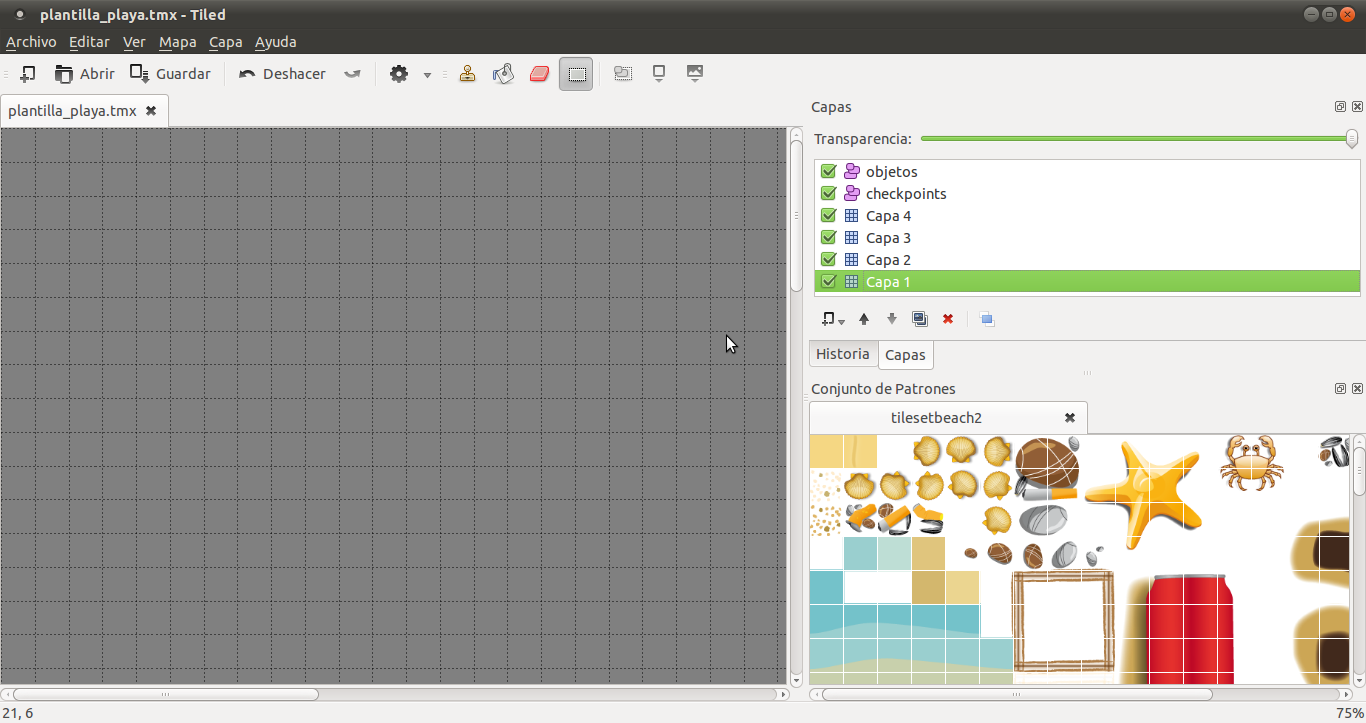
\includegraphics[scale=0.35]{imagenes/manualcircuito/interfaz_tiled.png}
  \end{flushleft}
  \caption{Manual para añadir circuitos: interfaz de tiled.}
\end{figure}

\paragraph{}
Podemos diferenciar 4 zonas claramente que se describirán en los siguientes apartados.

\subsubsection{Zona superior -- Barra de herramientas}

\paragraph{}
Aquí tendremos las distintas herramientas en referencia a la capa que nos encontremos en ese momento.

\paragraph{}
Si estamos en una capa de tiles, tendremos herramientas para poner tiles, rellenar con tiles, borrar tiles y selección de un 
conjunto de tiles, de izquierda a derecha.

\begin{figure}[H]
  \label{herramientas_tiles}
  \begin{center}
    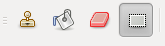
\includegraphics[scale=1]{imagenes/manualcircuito/herramientas_tiles.png}
  \end{center}
  \caption{Manual para añadir circuitos: herramientas capa de tiles.}
\end{figure}

\paragraph{}
Si la capa es de objetos, tendremos las herramientas de seleccionar objetos, insertar objetos e insertar objetos de patrones,
de izquierda a derecha.

\begin{figure}[H]
  \label{herramientas_objetos}
  \begin{center}
    
\includegraphics[scale=1]{imagenes/manualcircuito/herramientas_objetos.png}
  \end{center}
  \caption{Manual para añadir circuitos: herramientas capa de objetos.}
\end{figure}

\subsubsection{Zona izquierda -- Lienzo}

\paragraph{}
Esta será la zona donde iremos dibujando el circuito con los tiles disponibles en el tileset. Podremos hacer uso de las capas
para poder situar elementos por encima de otros y crear sensación de lejanía.

\paragraph{}
Podremos usar zoom in y zoom out con la rueda del ratón a la vez que pulsamos la tecla cntrl.

\subsubsection{Zona derecha-superior -- Capas}

\paragraph{}
En esta otra parte de la interfaz, tendremos las distintas capas que dispondremos para crear el circuito. Se pueden añadir
el número de capas que se desee, pero en la realización de circuito para \emph{Zycars}, sólo usaremos las que se ven en la imagen 
a continuación:

\begin{figure}[H]
  \label{capas}
  \begin{center}
    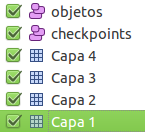
\includegraphics[scale=1]{imagenes/manualcircuito/capas.png}
  \end{center}
  \caption{Manual para añadir circuitos: Capas.}
\end{figure}

\paragraph{}
Podemos diferenciar entre dos tipos de capas, las capas de tiles, donde dibujaremos los tiles que tengamos en el tileset y la 
capa de objetos, donde marcaremos donde se situarán alguno objetos necesarios
de carreras, como pueden ser las cajas de ítems
o los puntos de control de la carrera.

\paragraph{}
El papel de cada una de ellas es el siguiente:

\begin{itemize}
    \item \textbf{Capa 1}: capa que sirve para situar el fondo del circuito
    \item \textbf{Capa 2}: capa donde podremos los tiles atravesables formando el recorrido del circuito y tiles de decoración.
    \item \textbf{Capa 3}: aquí podremos tiles que queramos que se vean por encima de los jugadores.
    \item \textbf{Capa 4}: sin uso actualmente.
    \item \textbf{Checkpoints}: capa de objetos donde podremos los puntos de control del circuito.
    \item \textbf{Objetos}: capa de objetos donde podremos las cajas de ítems y los puntos de la inteligencia artificial.
\end{itemize}

\subsubsection{Zona derecha-inferior -- Tileset}

\paragraph{}
En esta zona tendremos el tileset, es decir, la imagen que contiene el conjunto de tiles con el que crearemos el circuito.
Al igual que en el lienzo, podremos hacer zoom in y zoom out con la ayuda de la rueda del ratón mientras pulsamos la tecla
cntrl.

\subsection{Tipos de tiles.}

\paragraph{}
Antes de comenzar deberemos diferenciar claramente los distintos tipos de tiles que existen en \emph{Zycars}:

\begin{itemize}
    \item \textbf{Atravesables}: son los tiles usados para añadir decoración al circuito, como fondo u otros elementos.
    \item \textbf{Colisionables}: aquellos tiles que el jugador no podrá atravesar, se usarán para hacer el trazado del circuito
    y añadir obstáculos en este.
    \item \textbf{Realentizadores}: tiles por los que al pasar por encima
    ralentizarán considerablemente la velocidad del jugador.
\end{itemize}

\paragraph{}
Para diferencia bien cada uno de los distintos tipos, en la carpeta zycars/multimedia/image/, tenemos una imagen de guia, sólo
y únicamente sirve de guia, para saber de que tipo son los distintos tiles del tileset. En el caso de la playa, que es el que nos
ocupa, la imagen se llama mixedbeach.png, en el caso del jardín y la cocina mixedgarden.png y mixedkitchen.png, respectivamente.
A continuación un ejemplo de este tipo de imagen:

\begin{figure}[H]
  \label{mixed_beach}
  \begin{center}
    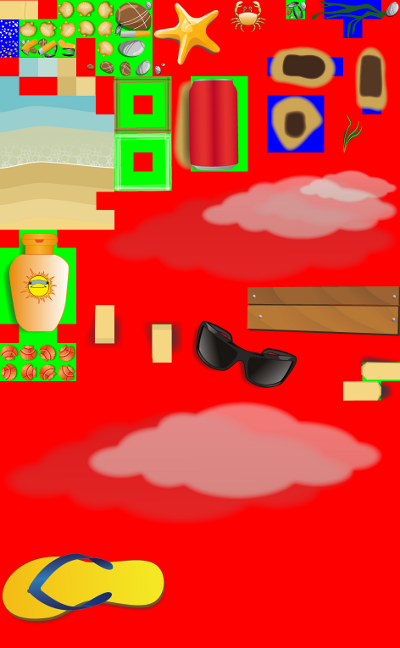
\includegraphics[scale=0.4]{imagenes/manualcircuito/mixedbeach.png}
  \end{center}
  \caption{Manual para añadir circuitos: Tileset con los tipos de tiles reflejados.}
\end{figure}

\paragraph{}
Como se puede ver e la imagen, tenemos 3 tipos de colores, para los tres tipos de tiles:

\begin{itemize}
    \item \textbf{Rojo}: indican los tiles atravesables
    \item \textbf{Verdes}: indican los tiles colisionables
    \item \textbf{Azules}: indican los tiles que ralentizan
\end{itemize}

\paragraph{}
Una vez aclarado los distintos tipos de tiles que encontraremos para cada circuito, ya estamos preparados para comenzar la creación
de circuitos.

\subsection{Añadiendo el fondo. Capa 1.}

\paragraph{}
En primer lugar nos centraremos en la capa 1, en esta capa podremos el fondo
del escenario, es conveniente que no pongamos ningún 
tile colisionables, nos centraremos únicamente en los tiles atravesables.

\paragraph{}
Por lo que en primer lugar deberemos seleccionar la capa 1 en ventana de capas, para indicar que vamos a comenzar a pintar en esa
capa. Una vez hecho esto, podremos empezar a rellenar el fondo del circuito. Para ellos tenemos muchos tiles con aspecto de arena,
de distintos tonos para diferenciar entre arena mojada y arena seca.

\paragraph{}
El resultado que obtendríamos sería el siguiente:

\begin{figure}[H]
  \label{circuito_fondo2}
  \begin{center}
    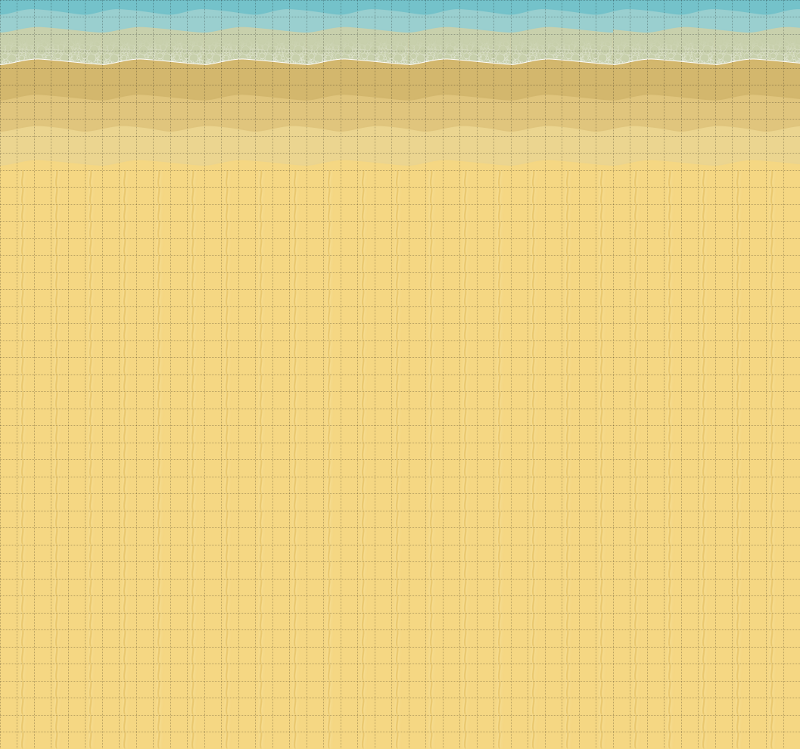
\includegraphics[scale=0.5]{imagenes/manualcircuito/circuito_fondo2.png}
  \end{center}
  \caption{Manual para añadir circuitos: Fondo circuito.}
\end{figure}

\paragraph{}
Una vez hecho el fondo de nuestro circuito, podremos pasar al siguiente paso, en el siguiente paso nos centraremos en realizar el 
trazado de nuestro circuito, donde competirán los distintos jugadores.

\subsection{Añadiendo trazado circuito. Capa 2.}

\paragraph{}
Para comenzar con el trazado del circuito, debemos seleccionar la capa 2. Antes de comenzar debemos fijarnos bien cuales de los 
tiles son colisionables, ya que el trazado siempre se realizara con tiles colisionables para que los jugadores no se puedan salir
del circuito.

\paragraph{}
En el caso concreto de la playa, tenemos distinto tiles para realizar el trazado, como conchas tanto amarillas, como rojas o las 
lineas marrones y blancas del tileset. Una vez claro los tiles disponibles, podemos comenzar a dibujar el trazado.

\paragraph{}
Se recomienda que todo el trazado del circuito tenga el mismo ancho, el todos los circuitos que ya existen en \emph{Zycars}, se usa
normalmente un ancho de 5 tiles para las pistas. Debemos tener claro el ancho máximo de la pista, ya que posteriormente deberemos
señalarlo en las opciones del circuito.


\paragraph{}
Un ejemplo de un posible trazado se muestra a continuación:

\begin{figure}[H]
  \label{circuito_trazado}
  \begin{center}
    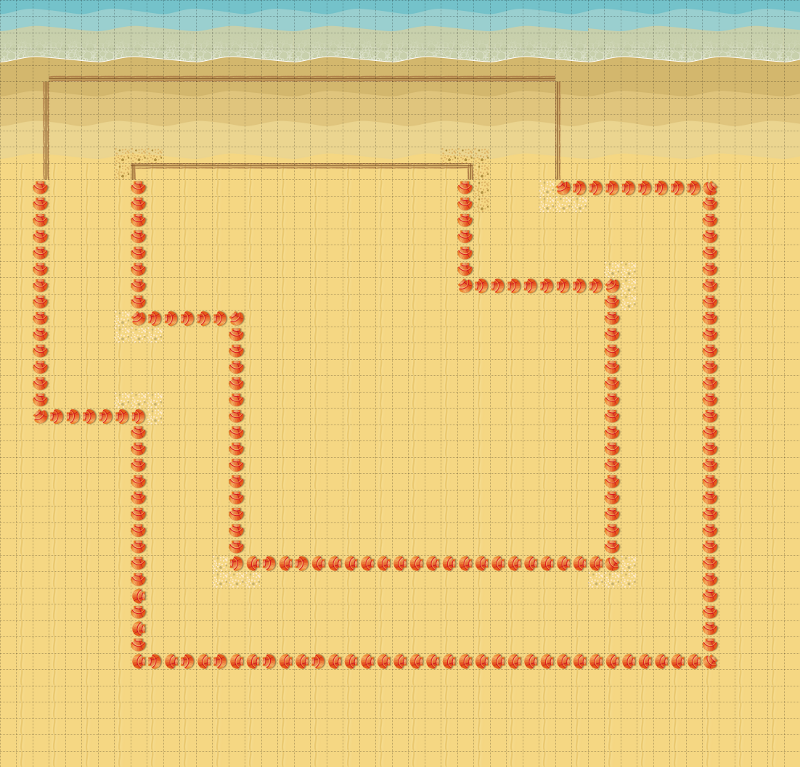
\includegraphics[scale=0.5]{imagenes/manualcircuito/circuito_trazado.png}
  \end{center}
  \caption{Manual para añadir circuitos: Trazado circuito.}
\end{figure}

\paragraph{}
Bueno tras este paso, ya tenemos lo más esencial de cualquier circuito que se precie. En el siguiente paso añadiremos elementos
de decoración por todo el mapa y obstáculos, para hacer más atractivo el
trazado del circuito y más ameno a la hora de 
competir en él.

\subsection{Añadiendo decorado. Capa 2.}

\paragraph{}
En esta sección y como se ha comentado en la sección anterior, nos dedicaremos
ha añadir obstáculos en el circuito, como pueden ser
tiles que ralenticen la velocidad de los jugadores u objeto colisionables en medio del trazado del circuito. Como podemos ver en
el tileset que estamos usando, tiles realentizadores son aquellos que parecen
manchas de humedad o los tiles que tiene un conjunto 
de pequeñas piedras.

\paragraph{}
También añadiremos objetos de decoración fuera del circuito, para hacer al escenario más agradable y vistoso. Tiles de adorno,
tenemos las gafas de sol, la chancla o por ejemplo la lata de refresco.

\paragraph{}
Para añadir el decorado y obstáculos seguiremos en la capa 2, con cuidado de no reemplazar los tiles que representan el trazado.
Un ejemplo de resultado obtenido sería el siguiente:

\begin{figure}[H]
  \label{circuito_decorado}
  \begin{center}
    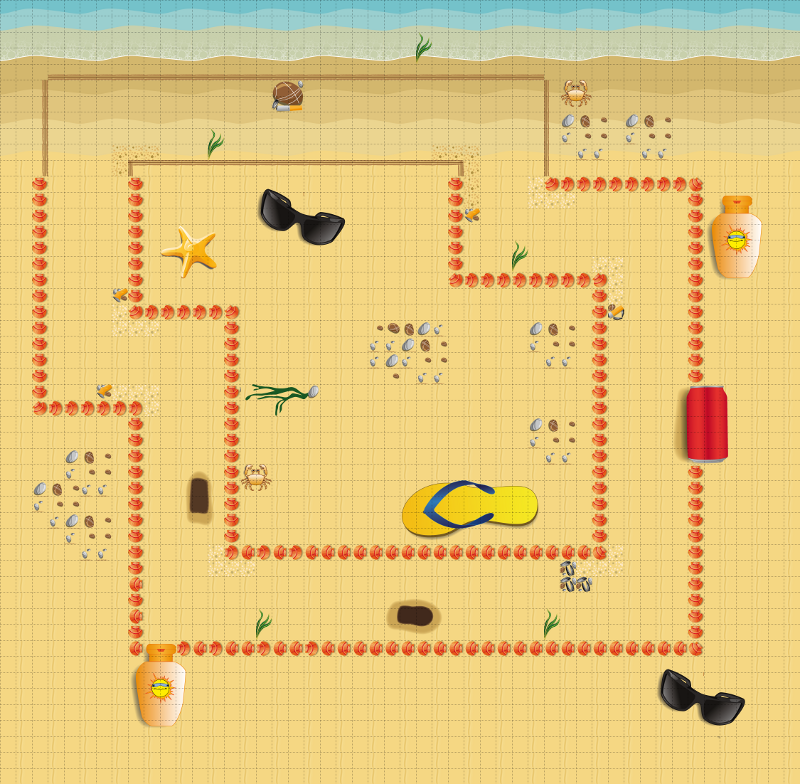
\includegraphics[scale=0.5]{imagenes/manualcircuito/circuito_decorado.png}
  \end{center}
  \caption{Manual para añadir circuitos: Decorado circuito.}
\end{figure}

\subsection{Añadiendo elementos superiores. Capa 3.}

\paragraph{}
El último paso en el que añadiremos tiles al circuito, será en está sección, donde añadiremos, si lo deseamos, aquellos elemento
que deseamos que se vean por encima de los jugadores.

\paragraph{}
En este tileset en cuestión, tenemos tiles que representan nubes, por lo que son lo ideal para añadir en esta capa 3. El resultado
quedaría de la siguiente forma.

\begin{figure}[H]
  \label{circuito_capa3}
  \begin{center}
    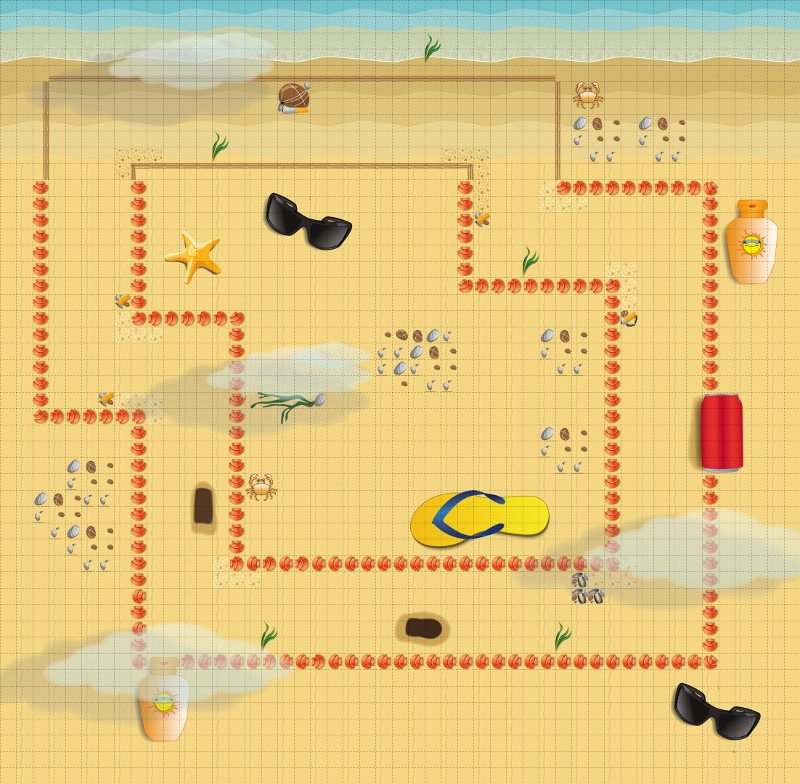
\includegraphics[scale=0.5]{imagenes/manualcircuito/circuito_capa3.png}
  \end{center}
  \caption{Manual para añadir circuitos: Capa 3 del circuito.}
\end{figure}

\paragraph{}
Una vez añadido los elementos de la tercera capa, hemos concluido la parte de creación y decoración del circuito. En las secciones
que vienen a continuación añadiremos todos los elementos necesarios para el correcto funcionamiento del juego en el nuevo circuito.
Por ello, en las siguiente secciones sólo trabajaremos con las capas de objetos.

\subsection{Rellenado la capa checkpoints.}

\paragraph{}
Como hemos comentado en la sección anterior, en las secciones que viene a continuación nos centraremos en añadir todos los 
objetos necesarios en el circuito. Trabajaremos con las capa de objetos y la de checkpoints disponible en la plantilla. 
Centrándonos en primer lugar en la capa de checkpoints.

\paragraph{}
Este puede ser uno de los pasos más importante y trabajosos a la hora de crear un circuito. En este paso, indicaremos donde se 
situará la meta y todos los puntos de control del circuito, que controlen que las vueltas se realizan de forma correcta.

\subsubsection{Indicando la salida.}

\paragraph{}
En primer lugar indicaremos donde estará la salida y meta del circuito, para ello seleccionamos la capa de checkpoints y 
situamos la meta donde queramos. Una aclaración si la meta va a ser horizontal se deberá colocar el objeto en la parte izquierda
del trazado, si en cambio es vertical, se deberá colocar en la parte superior del trazado. En este ejemplo la meta será horizontal,
su colocación será la siguiente:

\begin{figure}[H]
  \label{checkpoints1}
  \begin{center}
    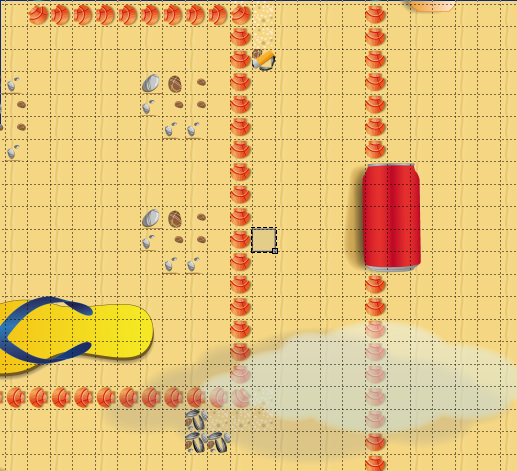
\includegraphics[scale=0.5]{imagenes/manualcircuito/checkpoints1.png}
  \end{center}
  \caption{Manual para añadir circuitos: Checkpoints paso 1.}
\end{figure}

\paragraph{}
Una vez que hemos añadido el objeto le damos el tamaño de un tile y pulsamos con el botón derecho del ratón sobre él y 
seleccionamos las propiedades del objeto. Ahora deberemos indicar que orientación que tiene en el atributo tipo, pondremos "GoalV"
si es vertical o "GoalH" si es horizontal. En el atributo nombre pondremos el valor 0, para indicar que es la salida. En nuestro
caso al ser la salida horizontal el resultado es el siguiente:

\begin{figure}[H]
  \label{checkpoints2}
  \begin{center}
    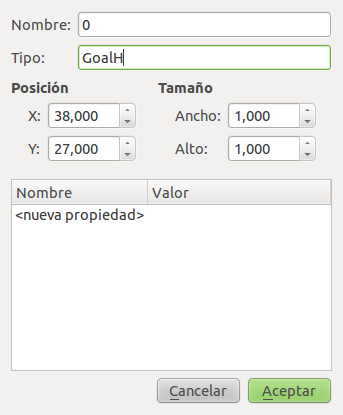
\includegraphics[scale=0.5]{imagenes/manualcircuito/checkpoints2.png}
  \end{center}
  \caption{Manual para añadir circuitos: Checkpoints paso 2.}
\end{figure}

\paragraph{}
Una vez añadido la salida, tendremos que indicar el ancho máximo de la pista, ancho de la pisa en la meta y la orientación en la 
que saldrán los jugadores, si hacia arriba(270)\footnote{Entre paréntesis se indica el valor que tendremos que añadir en función 
de la orientación}, abajo(90), izquierda(180) o derecha(0). En este caso a ser la salida horizontal, 
los jugadores sólo podrán salir hacia arriba o abajo. Por lo que en la parte superior de Tiled seleccionamos Mapa y propiedades 
del mapa y completamos las propiedades necesarias, que son "ancho\_meta" cuyo valor será 5, "ancho\_pista" que también será 5 y 
"grado\_coche" que deberá ser en nuestro caso 90 o 270. Para este ejemplo se ha elegido que los jugadores saldrán hacia arriba por lo
que daremos el valor 270.

\begin{figure}[H]
  \label{checkpoints3}
  \begin{center}
    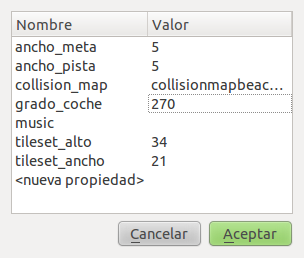
\includegraphics[scale=0.5]{imagenes/manualcircuito/checkpoints3.png}
  \end{center}
  \caption{Manual para añadir circuitos: Checkpoints paso 3.}
\end{figure}

\subsubsection{Añadiendo puntos de control.}

\paragraph{}
Una vez que hemos indicado donde se encontrará la salida y en que orientación saldrán los jugadores, deberemos añadir todos los
puntos de control necesario para el control correcto de las vueltas.

\paragraph{}
En este caso a la salir los jugadores hacia arriba empezaremos a añadir objetos por encima de la meta. Esto puntos de control
deberán cumplir las mismas reglas de la meta, a la izquierda del trazado cuando sean horizontales y en la parte superior cuando
sean verticales. Por encima de la meta iremos añadiendo objetos, poniendo en el tipo "Horizontal" y el nombre el número que 
corresponda, partiendo que el primero añadido será el 1. Quedando de la siguiente forma:

\begin{figure}[H]
  \label{checkpoints4}
  \begin{center}
    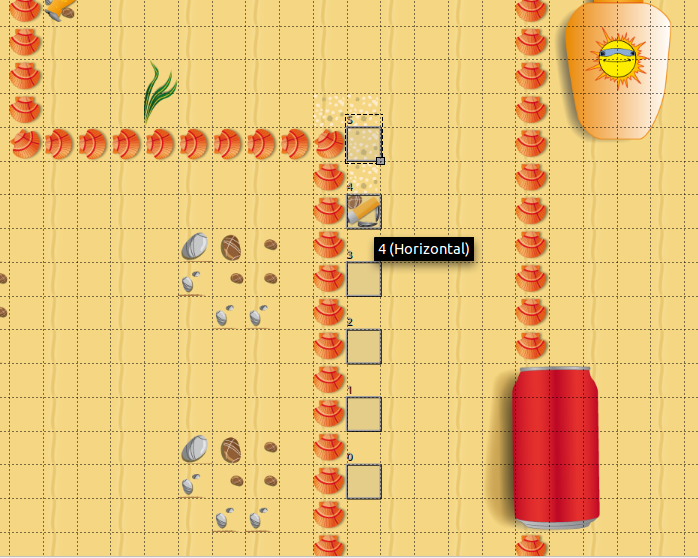
\includegraphics[scale=0.5]{imagenes/manualcircuito/checkpoints4.png}
  \end{center}
  \caption{Manual para añadir circuitos: Checkpoints paso 4.}
\end{figure}

\paragraph{}
Para los puntos de control verticales, un ejemplo de como quedaría:

\begin{figure}[H]
  \label{checkpoints5}
  \begin{center}
    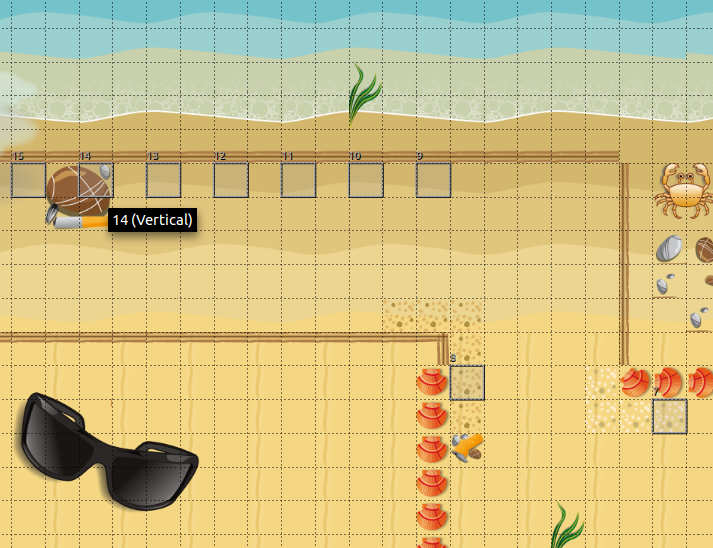
\includegraphics[scale=0.5]{imagenes/manualcircuito/checkpoints5.png}
  \end{center}
  \caption{Manual para añadir circuitos: Checkpoints paso 5.}
\end{figure}


\paragraph{}
Siguiendo los mismos pasos, deberemos añadir los puntos de control a lo largo de todo el trazado completo, siguiente la orientación
de este hasta llegar de nuevo a la salida de este. Quedando como resultado la siguiente imagen:

\begin{figure}[H]
  \label{checkpoints6}
  \begin{center}
    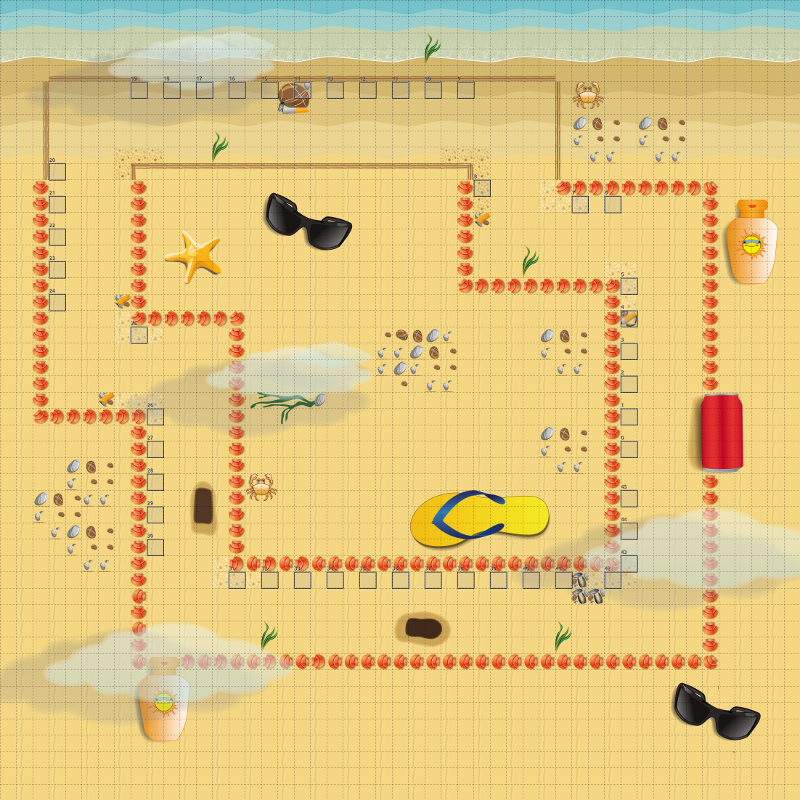
\includegraphics[scale=0.5]{imagenes/manualcircuito/checkpoints6.png}
  \end{center}
  \caption{Manual para añadir circuitos: Checkpoints paso 6.}
\end{figure}

\paragraph{}
Llegado a este punto ya hemos completado la introducción de todos los puntos de control necesarios en el circuito.

\subsection{Rellenado la capa objetos.}

\paragraph{}
En esta sección nos centraremos en añadir los distintos objetos necesarios en el circuito, como pueden ser, las cajas de ítem
y los puntos de control de la inteligencia artificial.

\subsubsection{Añadiendo cajas de ítems.}

\paragraph{}
Comenzaremos indicando mediante objetos donde se colocarán las cajas de ítems. Para ello nos situamos en la capa de objetos y 
seleccionamos en la barra de objetos añadir herramientas. Ahora hacemos click en alguna parte de escenario que esté dentro del
trazado del circuito. Tras hacer esto aparecerá un elemento transparente, al
que podremos dar el tamaño que deseemos (el tamaño no
afectará). Personalmente siempre le doy el tamaño de un tile, para que quede más claro.

\begin{figure}[H]
  \label{cajas_items1}
  \begin{center}
    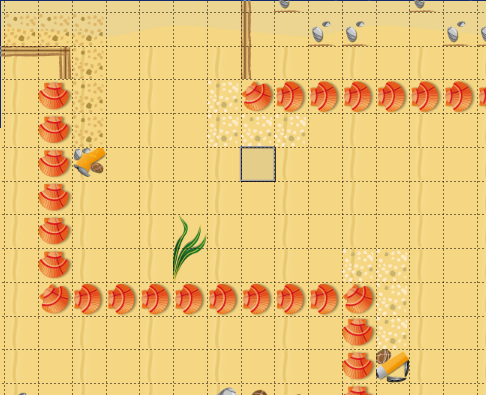
\includegraphics[scale=0.5]{imagenes/manualcircuito/cajas_items1.png}
  \end{center}
  \caption{Manual para añadir circuitos: Cajas de ítems paso 1.}
\end{figure}

\paragraph{}
Una vez lo tengamos como la imagen anterior, pulsamos con el botón derecho del ratón sobre este y seleccionamos "Las propiedades
del objeto". Una vez se nos habrá la ventana, añadiremos tanto en nombre como en tipo la palabra "Item\_box". Debe quedar como en la
siguiente imagen:

\begin{figure}[H]
  \label{cajas_items2}
  \begin{center}
    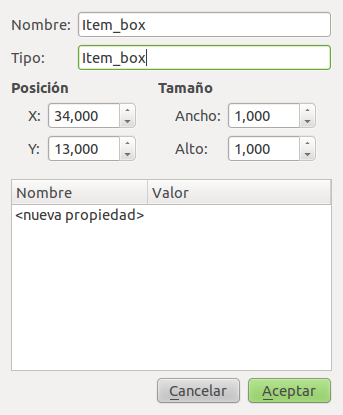
\includegraphics[scale=0.5]{imagenes/manualcircuito/cajas_items2.png}
  \end{center}
  \caption{Manual para añadir circuitos: Cajas de ítems paso 2.}
\end{figure}

\paragraph{}
Una vez hecho esto, solo nos quedará hacer lo mismo con tantas cajas de ítems que deseemos añadir. También podremos copiar el 
primer elemento e ir pegándolo por todo el circuito.

\subsubsection{Añadiendo control de la inteligencia artificial}

\paragraph{}
El último paso para completar la creación de nuestro circuito, será añadir los distintos puntos de control necesarios para que
la inteligencia artificial realice el recorrido correctamente. Para ellos deberemos añadir unos objetos en la capa de objetos, con
el tipo "check" y en el nombre el número correspondiente al punto de control comenzando desde 1. Añadiremos uno en cada curva del
circuito, siguiente el trazado de este en el orden en el que lo realizarán los jugadores. Quedando como resultado final la 
siguiente imagen:

\begin{figure}[H]
  \label{ia_check}
  \begin{center}
    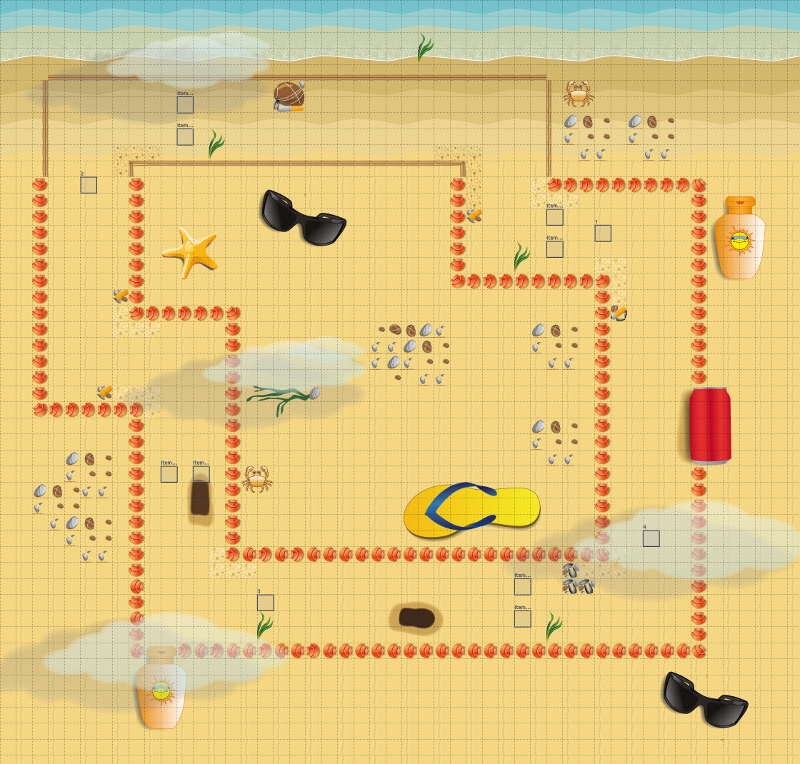
\includegraphics[scale=0.5]{imagenes/manualcircuito/ia_check.png}
  \end{center}
  \caption{Manual para añadir circuitos: Puntos de control de la inteligencia artificial.}
\end{figure}

\subsection{Modificando el xml generado.}

\paragraph{}
Una vez finalizado la creación del circuito, deberemos guardarlo en la carpeta "zycars/xml/circuits", que es donde se encuentran 
todos los circuitos del juego.

\paragraph{}
Tras hacer esto nos situamos en dicha carpeta y abrimos el archivo tmx generado al almacenar el circuito. Al inicio del xml,
aproximadamente en la línea 13, deberemos ver la siguiente línea:

\begin{lstlisting}[style=XML]
<image source="../../multimedia/image/tilesetbeach2.png" width="945" height="1530"/>
\end{lstlisting}

\paragraph{}
En esta línea deberemos borrar el siguiente trozo: "../../multimedia/image/", sin las comillas. Quedando de la siguiente forma:

\begin{lstlisting}[style=XML]
<image source="tilesetbeach2.png" width="945" height="1530"/>
\end{lstlisting}

\subsection{Añadiendo el mapa al juego.}

\paragraph{}
Por último, para añadir el circuito al juego, deberemos acceder al xml "fastracemenu.xml" que se encuentra en 
"zycars/xml/menu", una vez en el archivo deberemos buscar la etiqueta <layers>,
dentro de esta estarán las distintas capas
con los circuitos para cada uno de los campeonatos, si vamos añadir un circuito de playa nos centraremos en la capa cuyo atributo
name sea ''Copa Chancla'', si es un circuito de jardín será ''Copa arbusto'' y si es de cocina será ''Copa rodillo''.

\paragraph{}
Para cada una de ellas tenemos 4 circuito, por lo que deberemos sustituir el que queramos, modificando el atributo circuit\_file,
donde añadiremos el nombre del circuito que hemos creado. 

\paragraph{}
Por ejemplo si deseamos sustituir el primer circuito de la copa chancla:

\begin{lstlisting}[style=XML]
    <layers>
        <layer name="Copa Chancla" font_code="cheesebu" size="30">
            <buttons>
                <button type="image_button" xml_file="menu/circuitbutton.xml" 
                circuit_file='circuits/circuit1-beach.tmx' font="cheesebu" 
                text="circuit1-beach" image_circuit="circuit1" image="logo_beach1" 
                image_x="6" image_y="7" center="True" x="80" y="345" 
                show_text='False'></button>
\end{lstlisting}

\paragraph{}
Y el circuito que hemos creado se llama "mi\_circuito.tmx", debería quedar de la siguiente forma:

\begin{lstlisting}[style=XML]
    <layers>
        <layer name="Copa Chancla" font_code="cheesebu" size="30">
            <buttons>
                <button type="image_button" xml_file="menu/circuitbutton.xml" 
                circuit_file='circuits/mi_circuito.tmx' font="cheesebu" 
                text="circuit1-beach" image_circuit="circuit1" image="logo_beach1" 
                image_x="6" image_y="7" center="True" x="80" y="345" 
                show_text='False'></button>
\end{lstlisting}

\paragraph{}
Una vez hecho esto ya podremos disfrutar del circuito que hemos creado.
